\documentclass[10pt]{article}
\usepackage[paperwidth=8.5in,paperheight=11in,margin=.875in]{geometry}
\usepackage{fontspec}
\setmainfont{texgyretermes}[Extension=.otf,UprightFont=*-regular,BoldFont=*-bold,ItalicFont=*-italic,BoldItalicFont=*-bolditalic]
\usepackage{graphicx}
\usepackage{float}
\usepackage{caption}
\usepackage{parskip}
\pagestyle{plain}
\begin{document}
\section*{Full-width figure proof: 6.75 inches}
These figures describe the new native recurrent-language-model baseline, not the older frozen-vision-depth probe design. The primary status is illustrative. Real-model quality and H20/B300 performance are unmeasured.\par
\begin{figure}[H]
\centering
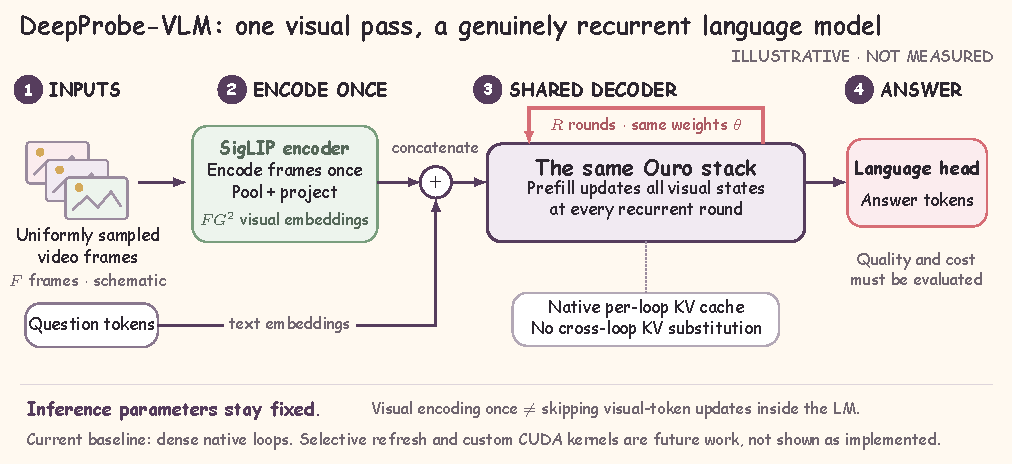
\includegraphics[width=6.75in]{../final/main_overview.pdf}
\caption{A single visual pass produces bounded visual embeddings, which enter the shared Ouro decoder alongside question embeddings. $F$ is the number of sampled frames, $G$ the pooled spatial grid size, and $R$ the native recurrent depth. The one return arrow denotes reuse of the language stack's weights. Visual states are updated during every recurrent prefill round; decoding retains the corresponding native per-loop KV caches. This does not establish cross-loop KV interchangeability, selective visual refresh, or an empirical improvement.}
\end{figure}\par
The dotted cache association is not a computation path. The frame glyphs are schematic vectors, not empirical video examples.
\clearpage
\section*{Training and evaluation proof}
\begin{figure}[H]
\centering
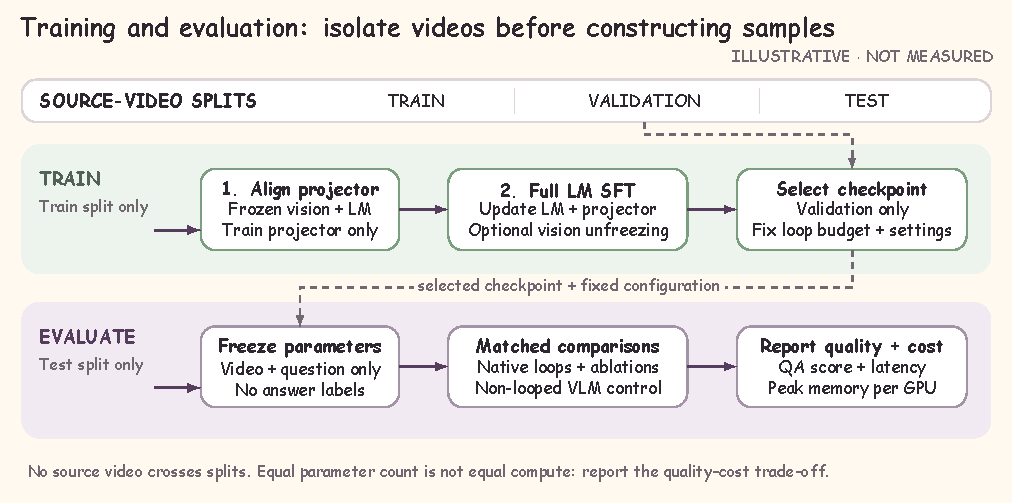
\includegraphics[width=6.75in]{../final/training_protocol.pdf}
\caption{Offline training and held-out inference occupy separate lanes. Alignment updates the pool/projector while freezing the backbones; the SFT stage updates the active language-model parameters and projector, with optional vision unfreezing. The unused adaptive exit gate remains frozen. Validation controls checkpoint and configuration selection; test labels are used only by the external scorer, never by inference. Source-video partitioning prevents clips from the same source appearing across splits. Protocol is illustrative; no trained checkpoint or benchmark result is implied.}
\end{figure}\par
The non-looped control requires equivalent data treatment and a separately trained comparison checkpoint. Equal parameter count is not equal inference compute.
\clearpage
\section*{Runtime experiment proof}
\begin{figure}[H]
\centering
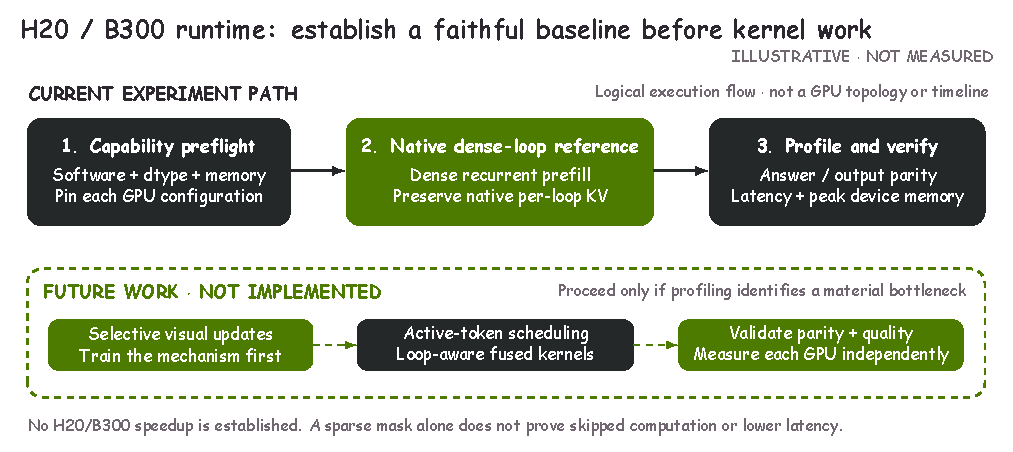
\includegraphics[width=6.75in]{../final/cuda_runtime.pdf}
\caption{A reference-first H20/B300 workflow. Solid arrows denote the dense native baseline path. The dashed group identifies conditional future work rather than shipped kernels: a selective-update mechanism must first be trained and validated, then scheduled efficiently. This is a logical software diagram, not a CUDA timeline, hardware topology, or profiler trace. H20 and B300 must be measured independently; neither speedup nor quality preservation has been established.}
\end{figure}\par
Dark green fills keep white labels readable on paper; color is redundant with the solid versus dashed grouping and the explicit future-work label.
\end{document}
